\documentclass[twocolumn]{article}

\usepackage{graphicx}
\usepackage{hyperref}
\usepackage{array}
\usepackage{booktabs}
\usepackage{caption}
\usepackage{float}
\usepackage{amsmath}

\title{%
    \vspace{-2cm}
    \textbf{Dine-Smart: \\ A Voice-Based Smart Assistant for Restaurant Searches and Reservations} \\
    \vspace{0.5cm}
    \large Implementation and Evaluation of a Rasa-Based Assistant
}

\author{
    Francesco Gentile (id. 240186) \\
    francesco.gentile@studenti.unitn.it \\
}

\date{}

\begin{document}

\maketitle

\section{Introduction}

This report outlines the development and implementation of Dine-Smart, a voice-based smart assistant built using Rasa and provided as an Alexa Skill. Dine-Smart serves as an intuitive voice-based interface over the Google Maps API, offering functionalities that include finding restaurants and bars, managing search results, making reservations, and handling existing reservations. It provides a seamless and engaging user experience by combining the extensive data capabilities of Google Maps with advanced conversational skills.

The project aims to enhance user convenience by providing an interactive and intelligent assistant for dining-related queries and tasks. By leveraging Natural Language Processing (NLP) techniques within the Rasa framework, Dine-Smart can understand and respond to user queries with accuracy and contextual relevance.

This report details the development process of Dine-Smart, including the capabilities and features of the assistant, the design and architecture of the system and the integration of Rasa with the Google Maps API. It also evaluates the performance of the assistant and user feedback, identifying successes and areas for improvement.

\section{Capabilities and Features}

Differently from existing voice-based assistants, like Alexa or Siri, Dine-Smart is not a general-purpose assistant but is specifically designed to assist users with dining-related queries and tasks. By combining task-based and information-retrieval functionalities, Dine-Smart can be seen as a mixed-initiative system, where the user and the assistant take control of the conversation interchangeably to achieve the desired outcome.

In developing Dine-Smart's conversational capabilities, I prioritized conciseness and efficiency in the design. The assistant is intentionally not overly talkative, delivering only the information requested by the user, with occasional additional details that are likely to be relevant. It asks only for the essential information needed to proceed, and where possible, it makes informed assumptions about what the user might be looking for to avoid excessive questioning. These assumptions are usually accurate, but the user has always the option to modify them.

This design choice was made with the understanding that many existing voice-based assistants can feel slow and less human-like, often frustrating experienced users with lengthy responses. To address this, Dine-Smart avoids long-winded explanations and uses implicit rather than explicit confirmations. For example, if a user indicates they are looking for a restaurant, the assistant might ask, ``Where would you like to look for restaurants?'' without requiring a direct confirmation of the initial request.

While this approach makes the conversation faster and more efficient, it also presents challenges. The interaction may feel less engaging, and new users might find it harder to navigate without more explicit guidance. To counter these potential issues, I have incorporated conversational markers to make the dialogue feel more natural and provide an option for users to request help. When asked, the assistant can offer guidance on specific tasks, such as how to conduct a search or make a reservation, or clarify what information the user can request or specify.

That said, in the following sections, I will describe the main conversational flows that Dine-Smart supports, highlighting the main features and capabilities of the assistant but also the limitations and areas for improvement.

\subsection{Search}

Dine-Smart’s core functionality revolves around helping users find restaurants, bars, and similar venues tailored to their preferences and location. The assistant supports a wide range of queries, allowing users to search for specific venues by name or more broadly by filtering according to criteria such as venue type, price, rating, cuisine, and the meal they plan to have (e.g., lunch, dinner, breakfast).

Consistent with the assistant’s design philosophy, Dine-Smart asks only for the essential information needed to perform a search using the Google Maps Places API's Text Search function. Generally, two key details are required: the location and the type of place the user is interested in.

The bot always asks for the location unless it can deduce that the user is searching for a nearby place. In such cases, it uses the user’s current location if available (future versions may retrieve this information automatically from the Alexa device); otherwise, it prompts for this information and temporarily stores it for the session.

As for the type of venue, the bot only inquires about this if it cannot make reasonable assumptions based on the user’s input. For example, if the user mentions they want to eat or have a drink, the bot can infer whether to search for a restaurant or a bar. Similarly,
if the user specify the meal they plan to have or the cuisine they are interested in, the bot can use this information to suggest relevant venues.

Dine-Smart also accommodates over-informative users by allowing them to specify multiple parameters simultaneously. This capability ensures that even if the user provides more information than what is currently requested, the search can proceed efficiently.

Once the required search parameters are set\footnote{Note that the user can also stop the search at any time, thus preventing the assistant from making the search or modifying the existing one.}, the search is saved to the user’s history. Users can then access this history to review previous searches, revisit specific entries, view detailed information, or delete past searches.

\subsection{Results}

After performing a search (or selecting a previous one from the history), Dine-Smart presents the user with a list of results, which can be navigated using voice commands. By default, the results are ranked by relevance, but the user has the option to sort them by distance if preferred.

The user can then request detailed information about these places, such as their location, ratings, price level, and opening hours. For convenience, Dine-Smart allows users to request this information for multiple places at once. However, the system currently does not allow users to request different types of information for the same or different places in a single command. This limitation exists because each type of information is linked to a distinct intent rather than an entity, due to the variety of ways users might phrase their queries. Supporting multiple information types simultaneously would necessitate defining all possible combinations of intents, which would result in an exponential growth in the complexity of the system.

\subsection{Reservations}

Dine-Smart offers two ways to make a reservation. In the first, the user selects a venue from their search results and requests to book it. In the second, if the bot detects that the user is likely searching with the intent to visit a venue, it will proactively ask if they want to reserve the place once it has been selected.

During the booking process, the bot prompts the user for the necessary details: the date and time of the reservation, the number of people, and the name under which the reservation should be made. It is important to note that, as the Google Maps API does not support actual bookings, the reservations made by Dine-Smart are simulated. The system only verifies that the venue can be reserved and that the chosen date is in the future. To enhance realism, there are also limitations on the maximum number of people and how far in advance a reservation can be made. As with searches, users can input all the required details simultaneously, without needing to wait for individual prompts from the bot.

After gathering all required information\footnote{As with searches, the user can stop the reservation process at any time, preventing the assistant from making the reservation or modifying the existing one.}, the bot will summarize the reservation details and seek confirmation — this is the only point in the conversation where explicit confirmation is used. Upon user confirmation, the booking is saved to their history. The user can then view and search their reservations, modify them, delete them, or check the details later.

\section{Technical Details}

To make the assistant independent of the Alexa platform or any other voice-based interface, Dine-Smart was implemented using the Rasa framework, an open-source platform for building conversational AI applications. Hereafter, I will describe how I leveraged Rasa to develop the assistant, focusing on the two main components of the system: the NLU pipeline and the dialogue management components.

\subsection{NLU Pipeline}

In Rasa and other conversational AI frameworks, the Natural Language Understanding (NLU) pipeline is responsible for processing user inputs and extracting structured information from them (i.e. entities and intents) that can be used by the dialogue management component to generate appropriate responses.

\subsubsection*{Data}

Due to the lack of existing datasets with conversations between users and voice-based assistants tailored for dining-related tasks, all training data were manually generated and annotated with intents and entities. This process involved creating a diverse and representative set of example interactions to train the model effectively.

To make sure that the assistant can understant the different nuances of user inputs (and act accordingly), 77 intents were defined. These many intents are necessary not only to cover the wide range of possible commands and queries that the user might issue, but also to better extract implicit information from the user's input. For example, if the user says ``i am hungry'', the assistant should be able to infer that the user is looking for a place to eat and they are looking for it now. Being able to extract this implicit information is crucial to allow the assistant to make informed assumptions and provide a more efficient and natural conversation. Since this information cannot be extracted from the user's input using entities, it is necessary to define specific intents for these cases. Similarly, filtering the search results by price or rating, as well as sorting the results by distance or relevance, can be expressed in multiple ways making it difficult to map them to a set of canonical entities, thus requiring specific intents to handle them.

Few intents have also been defined to handle out-of-scope requests, such as asking for the weather or the time, or to handle dining-related requests that the assistant cannot still handle, such as ordering food or drinks. When the assistant receives such requests, it will inform the user that it cannot handle them and suggest alternative ways to fulfill their needs.

Finally, to ensure the system's robustness and ability to generalize, more than 1500 examples were created. The distribution of examples among the intents is not uniform, with some intents having more examples than others, depending on their complexity and the variety of ways they can be expressed. On average, each intent has 19.5 examples, with a minimum of 11 examples and a maximum of 52. The same applies to entities, with 8 learnable and more than 800 examples in total. By having a diverse and representative set of examples, the assistant can handle different communication styles, including under-informative users (e.g., sentences with ambiguous entities), over-informative users (e.g., sentences with multiple entities), users that provide very short responses, and users that provide the required information surrounded by irrelevant information. To further support over-informative users, multi-intents were also defined, allowing the assistant to answer in a single turn to multiple user requests. Even if it is possible to automatically generate multi-intents by simply combining the examples of the single ones, I decided to manually define them only for the most likely combinations, so as to avoid their combinatorial explosion and to keep the training data manageable.

\subsubsection*{Components}

In developing the NLU pipeline for Dine-Smart using Rasa, I encountered challenges due to the large number of intents and the complexity involved in distinguishing among them. In particular, I found that using either hand-crafted featurizers or pre-trained language models was not sufficient to achieve satisfactory accuracy and generalization. Only by combining the two approaches was I able to achieve satisfactory results. Indeed, while the former allow the classifier to use more domain specific features, the latter enable it to leverage the knowledge extracted by large language models trained on large text corpora, thus capturing the nuances of user input more effectively.

The pipeline begings with a WhitespaceTokenizer, followed by sparse featurizers, i.e. the LexicalSyntacticFeaturizer and the CountVectorsFeaturizer (following the default Rasa configuration) and a dense featurizer based on the RoBERTa language model. These components are used to extract features from the user's input and pass them to the DIETClassifier, a transformer-based model that combines the extracted features to predict the intents and entities. To handle low-confidence predictions (below 0.2), a FallbackClassifier is incorporated, which triggers a rule prompting the user to rephrase their input. Additionally, a ResponseSelector is employed to manage help requests.

While this approach works well for grammatically correct inputs, it falters when typos or grammatical mistakes are present, as the training data is free of such errors. For example, the model confidently classifies ``I am hungry'' with a score of 0.95, but a simple typo like ``I am hugnry'' drops the score to 0.2. To address this issue without cluttering the training set with erroneous examples, I added a custom preprocessing component that uses the Bing SpellCheck API to correct typos, grammar errors, and slang, enabling the model to be trained and used on clean data.

For entity recognition, besides the DIETClassifier, I utilized the DucklingEntityExtractor for non-learnable entities. The spell checker is particularly beneficial here, as typos can prevent rule-based extractors from recognizing entities like dates, times, or numbers. Finally, to ensure that the venue types provided by users are relevant to dining, a custom component checks the extracted types. In particular, instead of using a predefined list of valid venues, I used an NLU-based approach where the definitions of the extracted entity are sourced from the Cambridge Dictionary, encoded using HuggingFace sentence transformers, and compared to the phrase ``places where people can eat or drink''. If the similarity exceeds a threshold (0.5), the venue type is accepted; otherwise, the user will be prompted to provide a different type.

\subsection{Dialogue Management}

The dialogue management component of Dine-Smart is responsible for determining the assistant's next action based on the user's latest input and the overall conversation context. This is achieved through a combination of machine learning models and finite-state automata, which are implemented using Rasa's rule-based policies, as well as custom actions and forms.

Specifically, two forms have been created to manage the search and reservation processes. These forms are used to collect the necessary information from the user in a structured way, ensuring that all required details are provided before proceeding with the search or reservation.

Beyond forms, 45 custom actions have been implemented to handle more complex dialogue scenarios. These actions allow the assistant to adapt the conversation flow based on the current state of the interaction. They also manage the conversation state, which is represented by 35 slots, by extracting and validating their values, and by updating them as the conversation progresses. Custom actions also play a key role in generating dynamic responses by populating more than 100 predefined utterances with data from the conversation state. This approach is essential for implicit confirmation, as it allows the assistant to reference user inputs in its responses without requiring explicit confirmation. To avoid repetitive interactions, multiple response variations have been defined, making the conversation more engaging.

\subsubsection*{Data}

As for the NLU component, the dialogue management model was trained on manually generated stories and rules that cover a wide range of possible interactions between the user and the assistant. These stories were designed to test the assistant's ability to handle different scenarios, including successful and unsuccessful conversations (the so called happy and unhappy paths), as well as edge cases and error handling.

In particular, a set of 44 rules and 44 stories was created to cover the main functionalities of the assistant, such as searching for a restaurant, making a reservation, checking the history, and handling errors. Following the Rasa guidelines, rules have been used to handle single turn interactions that do not require context (e.g. successful user commands or unrecoverable errors that do not require further user inputs), while stories have been used to handle multi-turn interactions that require context (e.g. unhappy paths where the assistant needs to ask for more information to complete the task). Furthermore, to make the training of the dialogue management model more efficient, shorter stories that focus only on one subtask at a time have been preferred over long stories that cover the whole conversation.

\subsubsection*{Policies}

Differently from the NLU pipeline, no particular expedients were taken when selecting the dialogue management model. Indeed, generating high quality training data, covering a wide range of possible interactions and scenarios, has proven to be much more effective in improving the model's performance than using more complex architectures or techniques. For such reasons, a similar pipeline to the one provided by Rasa was used, consisting of the AugmentedMemoizationPolicy, the RulePolicy (with fallback enabled), and the TEDPolicy.

\section{Evaluation}

To evaluate the performance of Dine-Smart, I conducted both intrinsic and extrinsic evaluations. While intrinsic evaluations uses objective metrics to assess the assistant's ability to understand and correclty respond to user inputs, extrinsic evaluations focus on the user experience and satisfaction with the assistant. In the following sections, I will describe the methodologies and results of both evaluations.

\subsection{Intrinsic}

Instrinsic evaluations have been carried out for both the NLU and dialogue management components of Dine-Smart.

For the NLU component, I evaluated both the adopted mixed approach, that combines deep-learning-based and traditional featurizers, and the default configuration provided by Rasa, that uses only hand-crafted featurizers. To ensure a reliable evaluation, I used a 10-fold cross-validation approach, splitting the training data into ten folds and training the model on nine folds while testing it on the remaining one. This process was repeated 10 times, with each fold serving as the test set once. The evaluation metrics used are accuracy, precision, recall and F1 score (in their macro-averaged form) for both intents and entities.

As can be seen from Table \ref{tab:intent-evaluation} and Table \ref{tab:entity-evaluation}, the mixed approach outperforms the default configuration in all metrics for both tasks. Still, the mixed approach also shows some limitations, in particular in the intent classification, where even the accuracy is below 80\%. As can be seen from the confusion matrices in the appendix, the model struggles to distinguish between intents that are strongly related to each other, such as the different intents to perform a search (that differ only in the implicit information that the user provides) or the intents that specify the quality and price range of the venue. However, I found that even humans can struggle to distinguish between these intents, thus suggesting that the model's performance is acceptable for the task at hand. As for the entity classification, the model seems to struggle in the extraction of entities, rather that in their classification, as the confusion matrix shows that the model often labels as entities words that are not and vice versa.

\begin{table}[ht]
    \centering
    \begin{tabular}{lcc}
        \toprule
        \textbf{Metric} & \textbf{Mixed} & \textbf{Default} \\
        \midrule
        Accuracy        & 79.40          & 71.51            \\
        Precision       & 80.19          & 72.56            \\
        Recall          & 78.91          & 72.60            \\
        F1 Score        & 78.87          & 71.45            \\
        \bottomrule
    \end{tabular}
    \captionsetup{margin=0.5cm}
    \caption{Evaluation metrics for intent classification using the mixed approach and the default configuration.}
    \label{tab:intent-evaluation}
\end{table}

\begin{table}[ht]
    \centering
    \begin{tabular}{lcc}
        \toprule
        \textbf{Metric} & \textbf{Mixed} & \textbf{Default} \\
        \midrule
        Accuracy        & 98.60          & 98.31            \\
        Precision       & 83.13          & 80.49            \\
        Recall          & 75.95          & 72.52            \\
        F1 Score        & 78.04          & 74.33            \\
        \bottomrule
    \end{tabular}
    \captionsetup{margin=0.5cm}
    \caption{Evaluation metrics for entity classification using the mixed approach and the default configuration.}
    \label{tab:entity-evaluation}
\end{table}

For the dialogue management component, a set of test stories was created to evaluate the assistant's ability to handle different scenarios and user inputs. The stories were designed to cover a wide range of possible interactions, including successful and unsuccessful conversations, as well as edge cases and error handling. In total, 10 test stories (for a total of 190 action predictions) have been created and used to evaluate the prediction accuracy of the dialogue management model. As reported in Table \ref{tab:dialogue-evaluation}, the model shows perfect accuracy in predicting the correct actions, thus demonstrating the effectiveness of the training data and the policies used.

\begin{table}[ht]
    \centering
    \begin{tabular}{lc}
        \toprule
        \textbf{Metric} & \textbf{Value} \\
        \midrule
        Accuracy        & 100.0          \\
        Precision       & 100.0          \\
        Recall          & 100.0          \\
        F1 Score        & 100.0          \\
        \bottomrule
    \end{tabular}
    \captionsetup{margin=0.5cm}
    \caption{Evaluation metrics for dialogue management on the test stories.}
    \label{tab:dialogue-evaluation}
\end{table}

\subsection{Extrinsic}

Extrinsic evaluations were conducted to assess the user experience and satisfaction with Dine-Smart. A group of 4 users was recruited to interact with the assistant and provide feedback on their experience. Each of these users was also paired with another observer, who was asked not to interact with the assistant but to observe the interaction and provide additional feedback. The participants were only given a brief introduction to the assistant and were asked to perform a series of tasks using Dine-Smart, such as searching for a restaurant, making a reservation, and checking their history. After completing the tasks, both the participants and the observers were asked to answer a series of questions to evaluate the assistant's performance and their satisfaction with the interaction.

As can be seen from Table \ref{tab:extrinsic-evaluation}, the overall satisfaction with the assistant was very positive, with an average rating of 4.3 out of 5. The functionalities provided by the assistant were also well-received, with users reporting high levels of satisfaction with the search and reservation capabilities. Participants have however raised some concerns about the history management functionalities that were perceived as less refined and less complete than the search and reservation functionalities. As for the assistant's design philosophy, which prioritizes conciseness and efficiency, it was highly appreciated by the participants and observers, who found the assistant to be fast and responsive in providing information and completing tasks.

\section{Conclusion}

In this report, I presented Dine-Smart, a voice-based smart assistant for dining-related queries and tasks. Despite the challenges faced during development, the assistant has demonstrated promising capabilities and features, providing users with an intuitive and efficient interface for finding restaurants, making reservations, and managing dining-related tasks.

Still, to make Dine-Smart an even more effective and engaging assistant, further improvements and refinements are needed. In particular, the NLU pipeline must be further extended and improved to better handle more complex user inputs and scenarios, in particular those cases in which the user changes their mind or provides conflicting information in the same utterance. Furthermore, new features and functionalities should be added to enhance the user experience and provide more value to users, such as the ability to order food or drinks, to provide more options for history management, or to integrate with other services and platforms.

\newpage

\onecolumn
\appendix

\section{Appendix}

\subsection{NLU Evaluation}

The following figures show the confusion matrices for the intent and entity classification tasks using the mixed approach and the default configuration. As can be seen, the mixed approach reports a lower number of false positives and false negatives, thus achieving better performance in both tasks.

\begin{figure}[H]
    \centering
    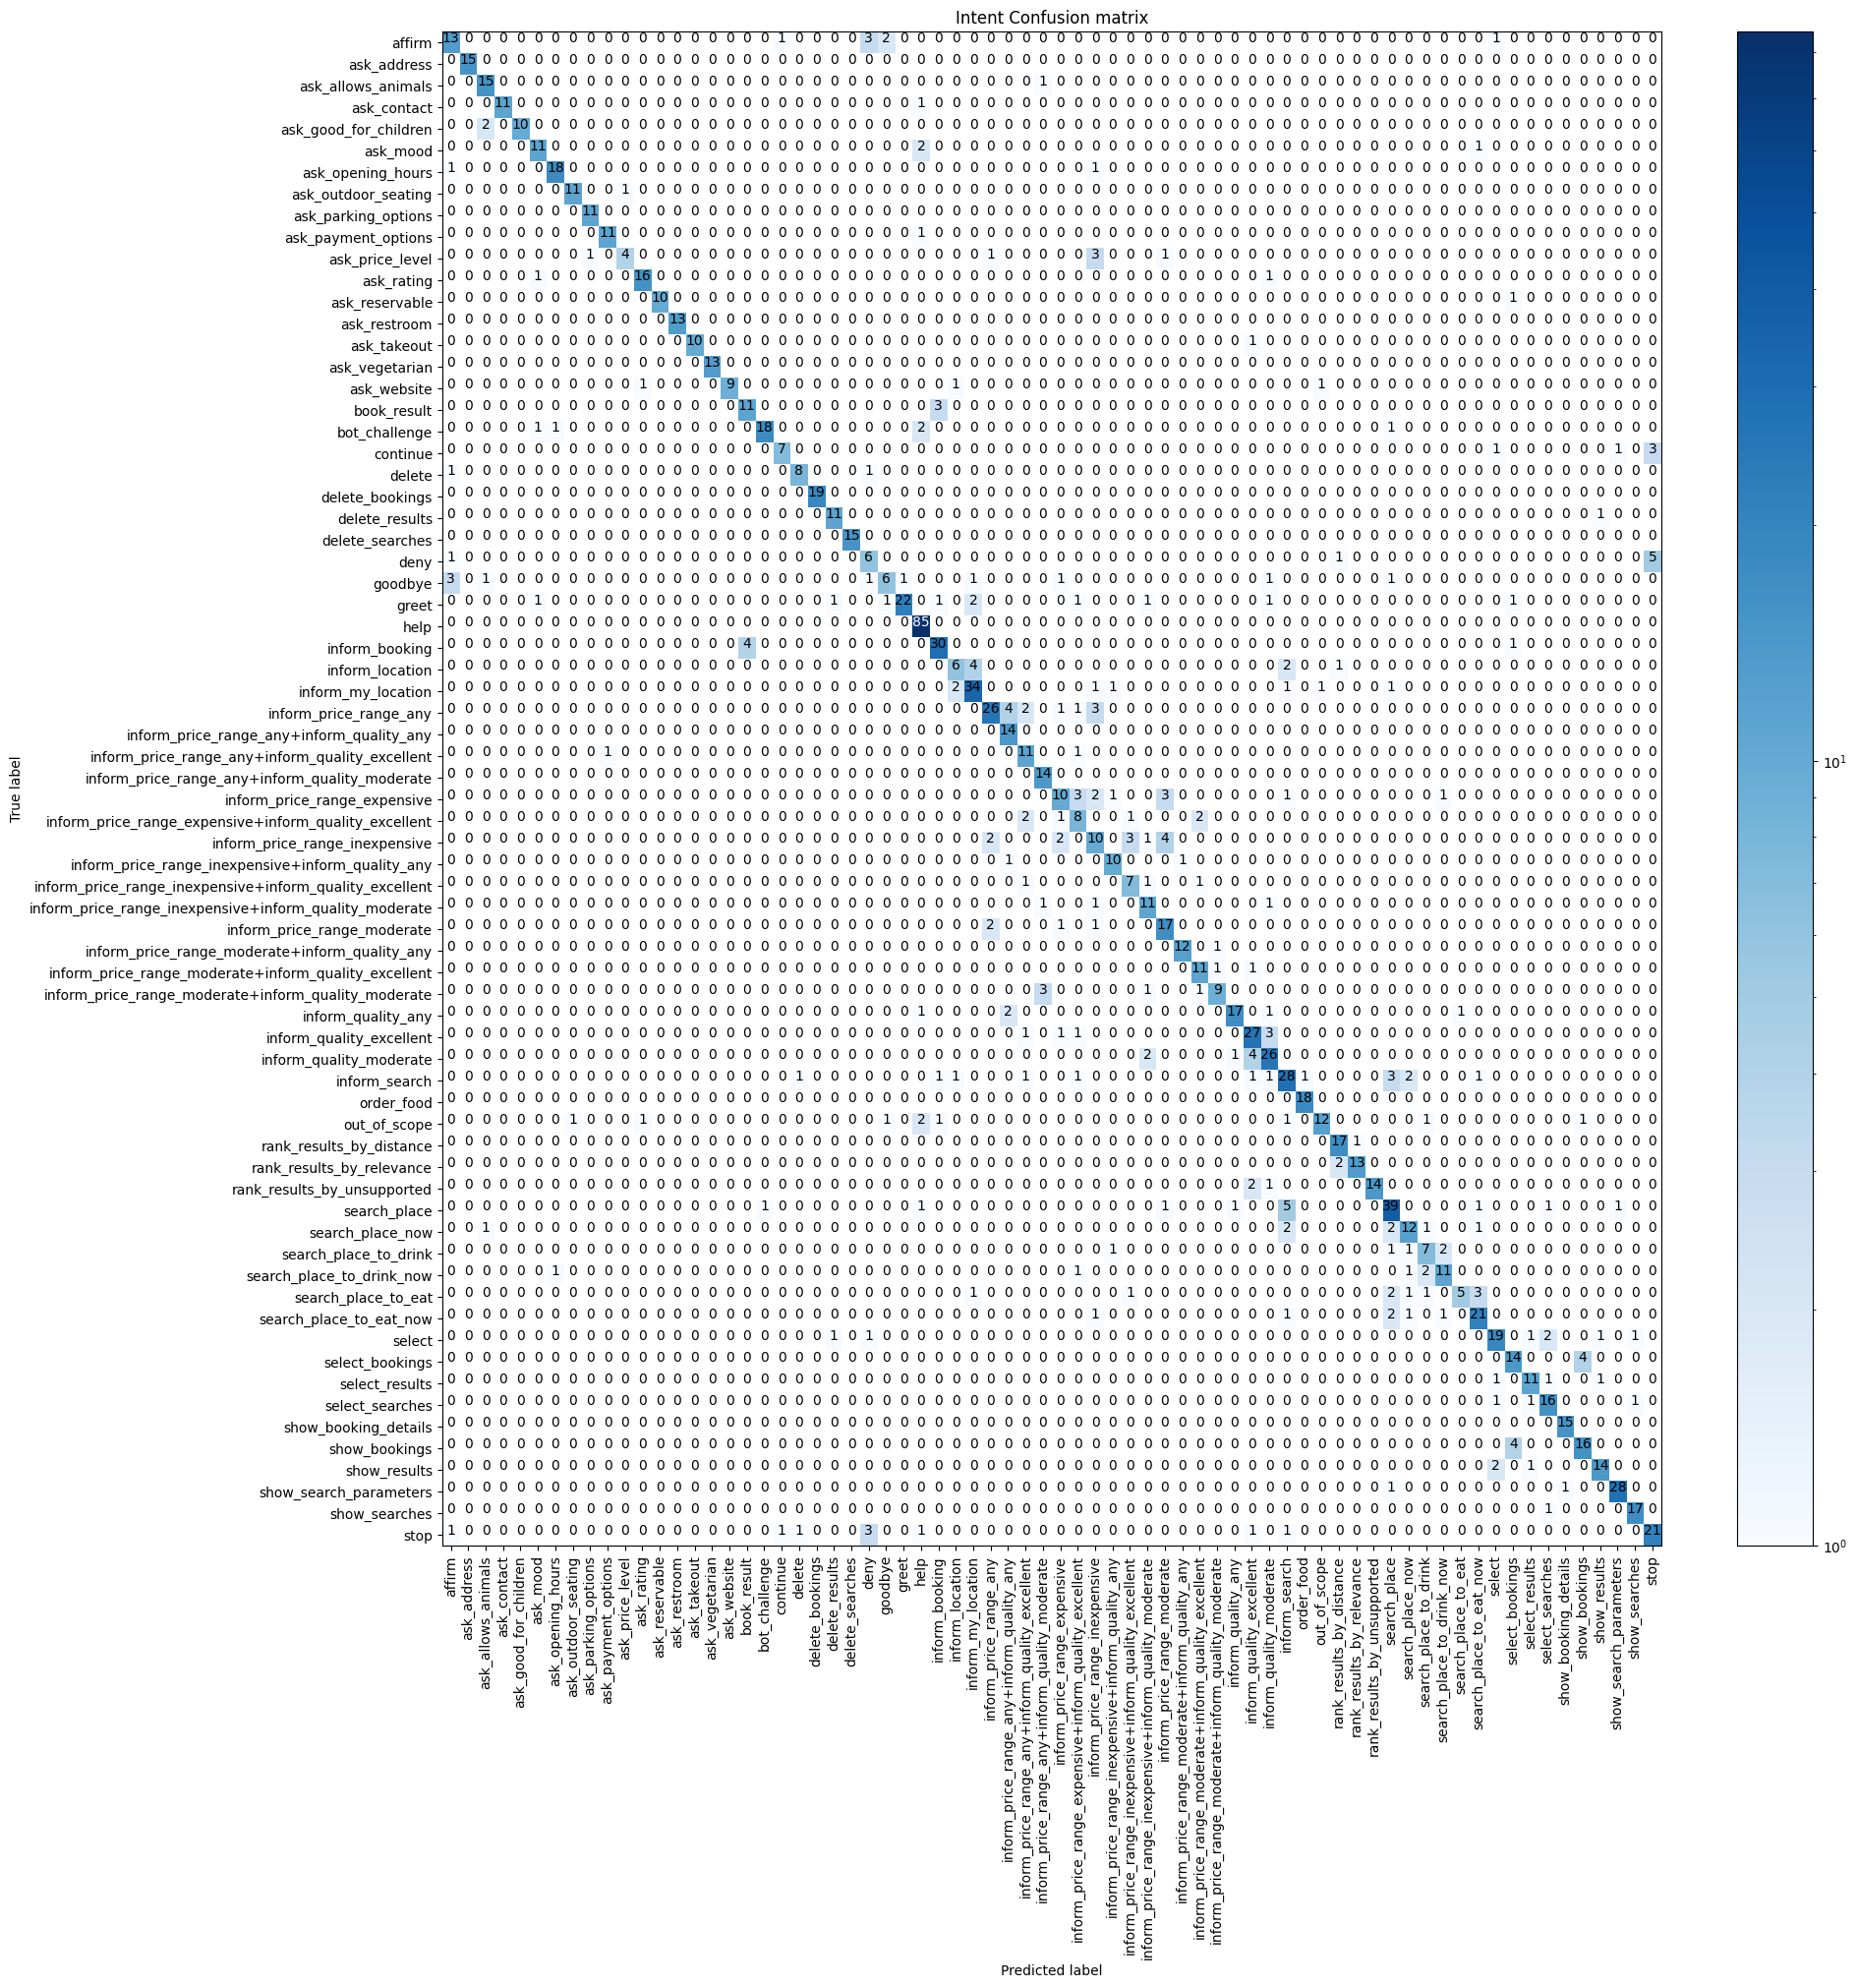
\includegraphics[width=0.8\textwidth]{images/intent_mixed_cf.png}
    \caption{Confusion matrix for the task of intent classification using the mixed approach.}
    \label{fig:intent-mixed-cf}
\end{figure}

\begin{figure}[H]
    \centering
    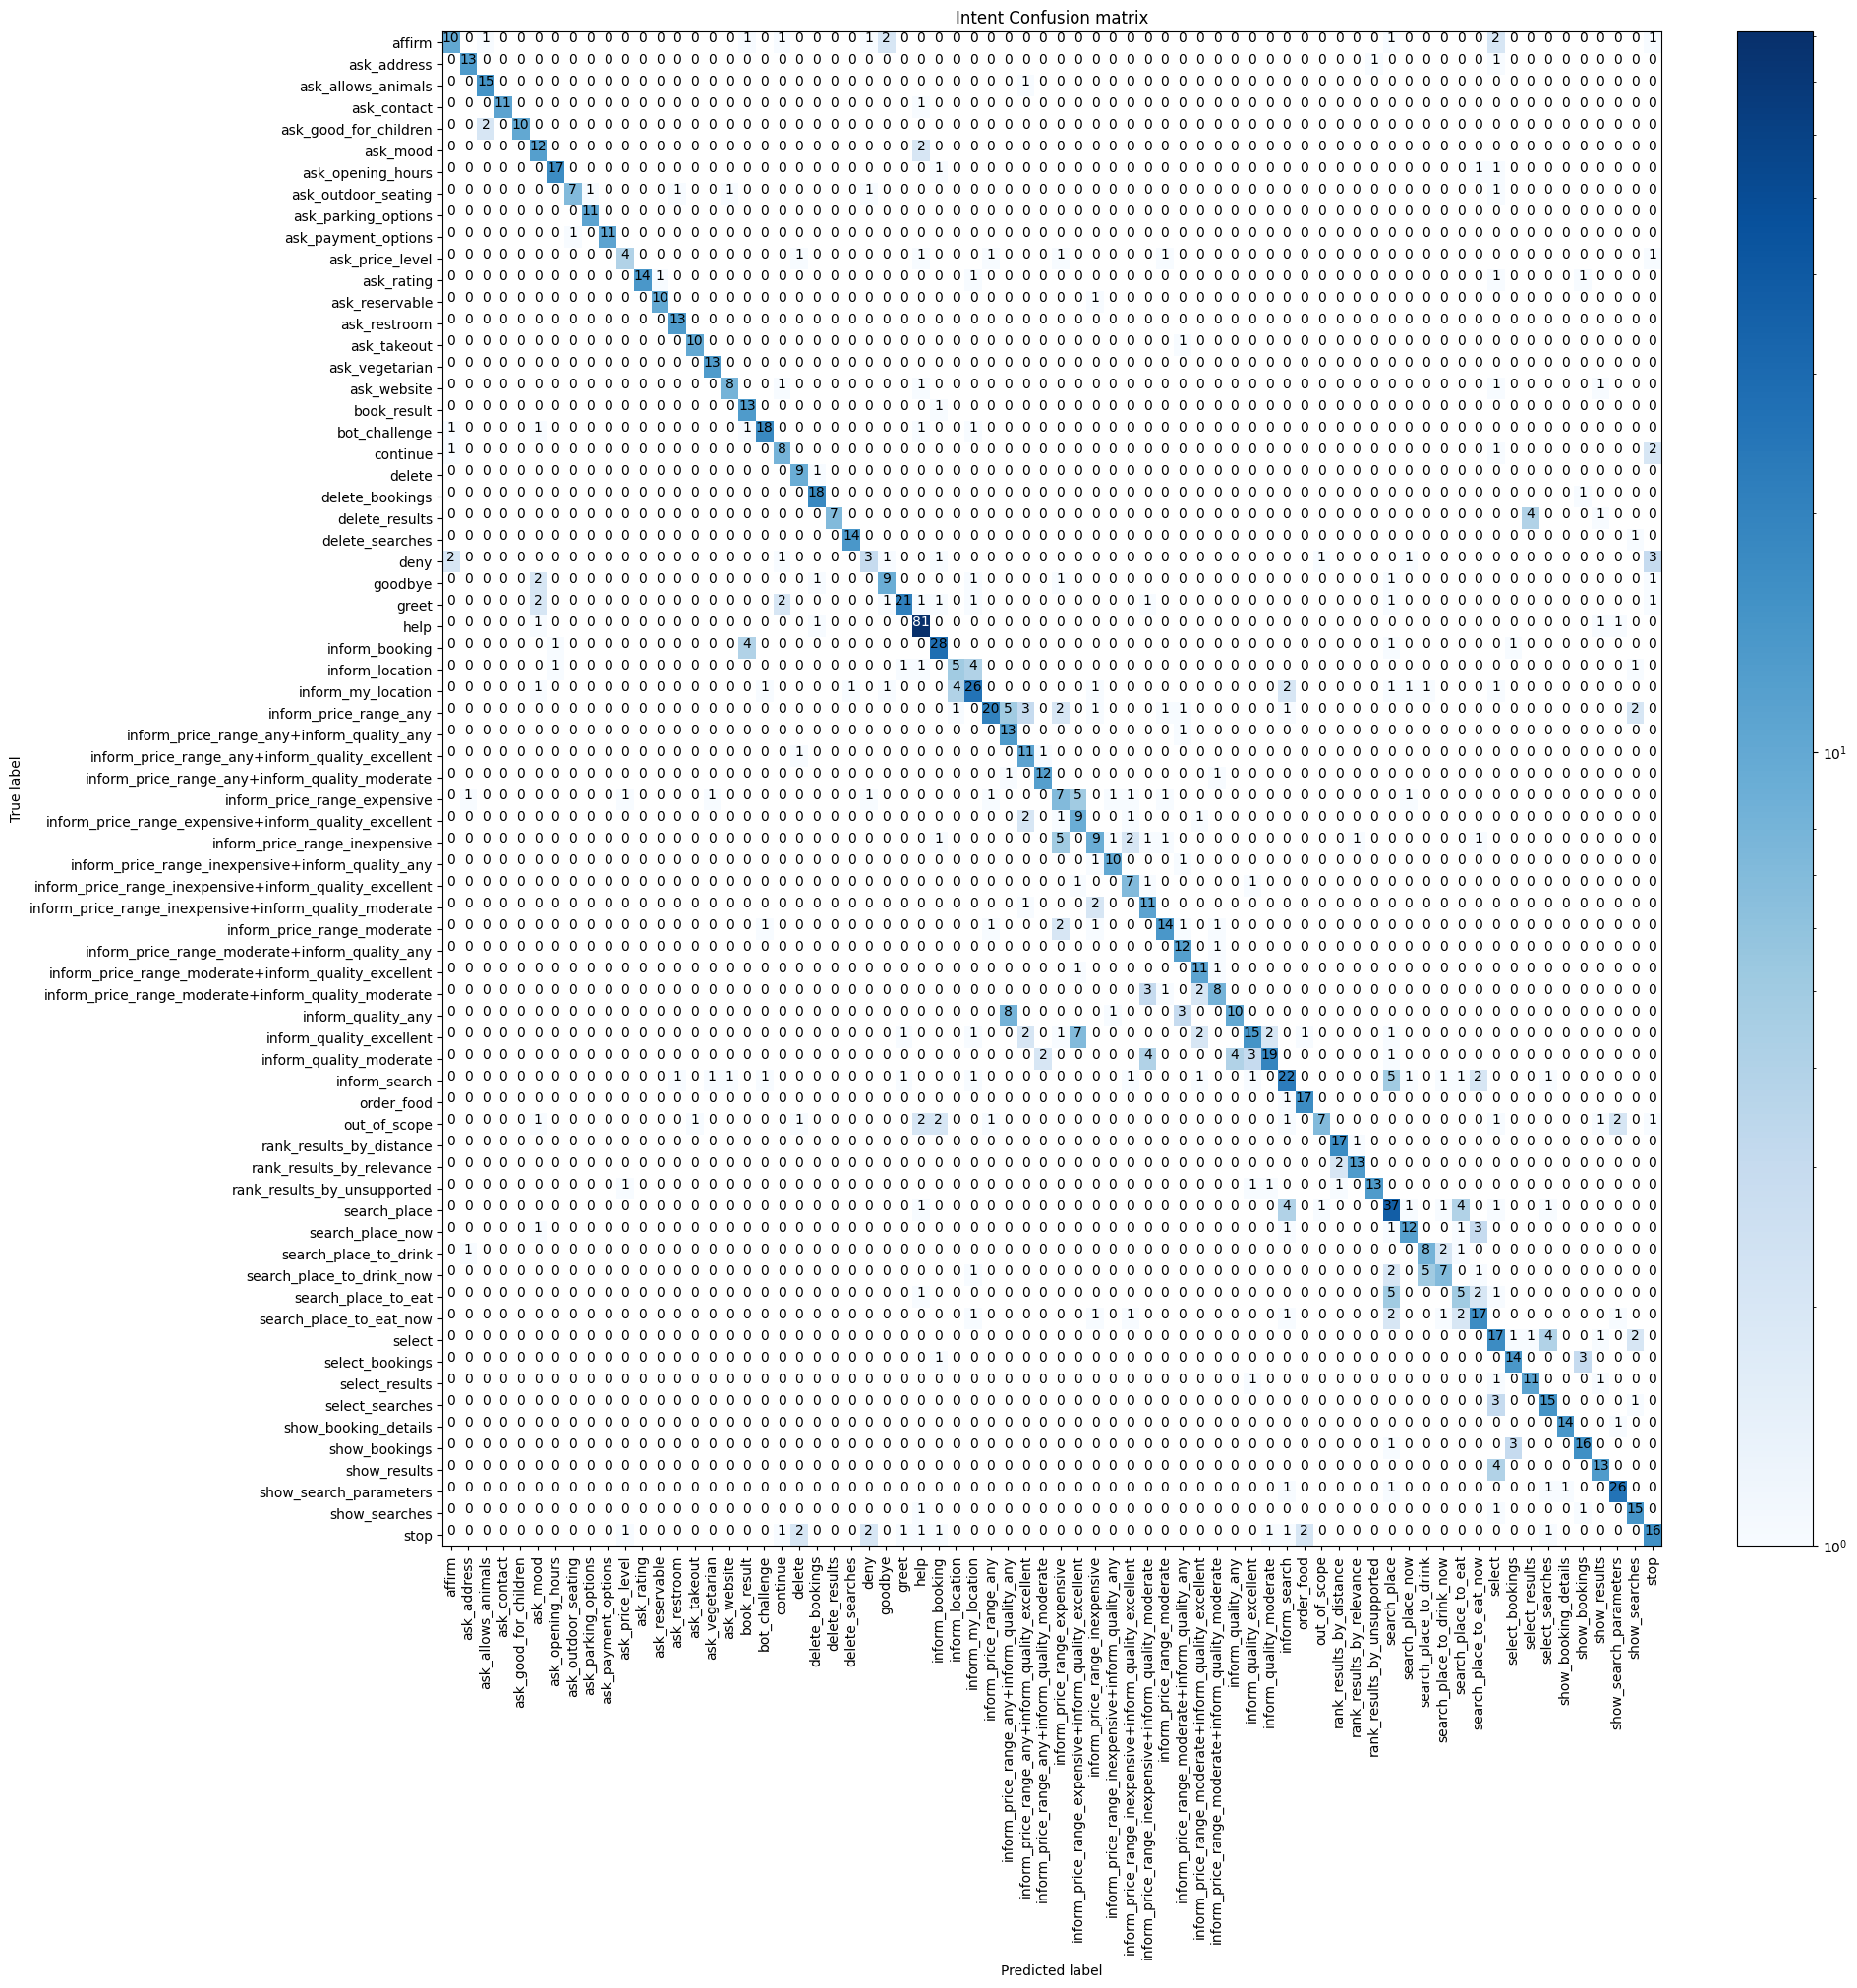
\includegraphics[width=0.8\textwidth]{images/intent_default_cf.png}
    \caption{Confusion matrix for the task of intent classification using the default configuration.}
    \label{fig:intent-default-cf}
\end{figure}

\begin{figure}[H]
    \centering
    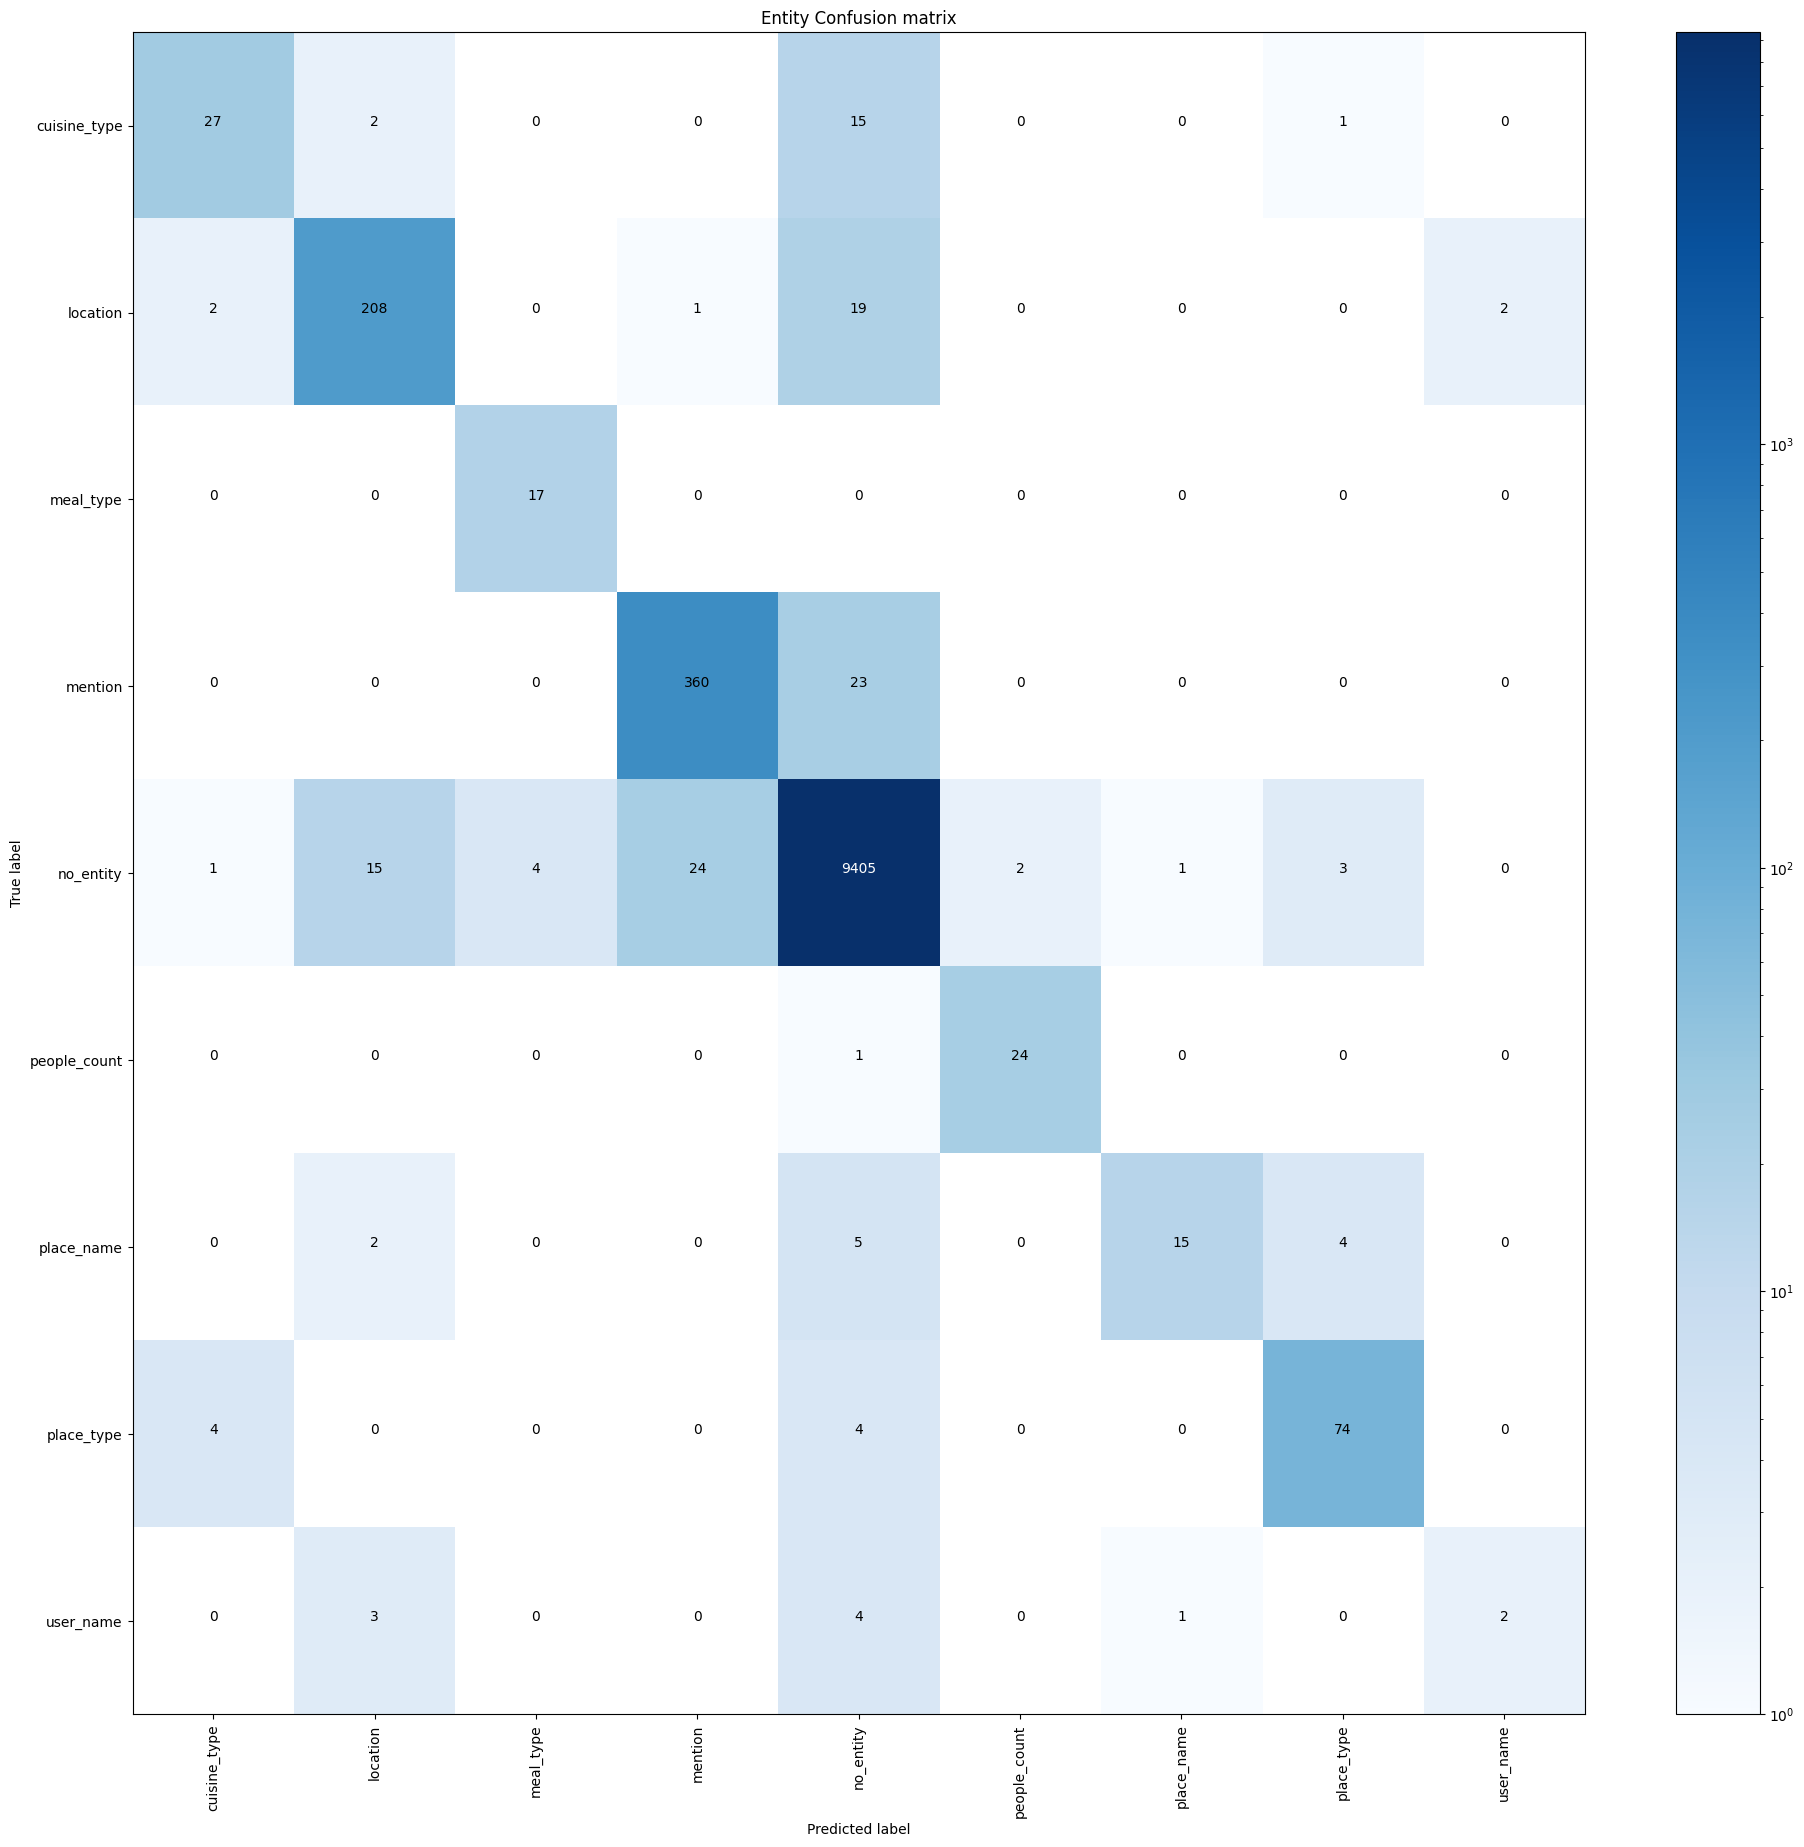
\includegraphics[width=0.8\textwidth]{images/entity_mixed_cf.png}
    \caption{Confusion matrix for the task of entity classification using the mixed approach.}
    \label{fig:entity-mixed-cf}
\end{figure}

\begin{figure}[H]
    \centering
    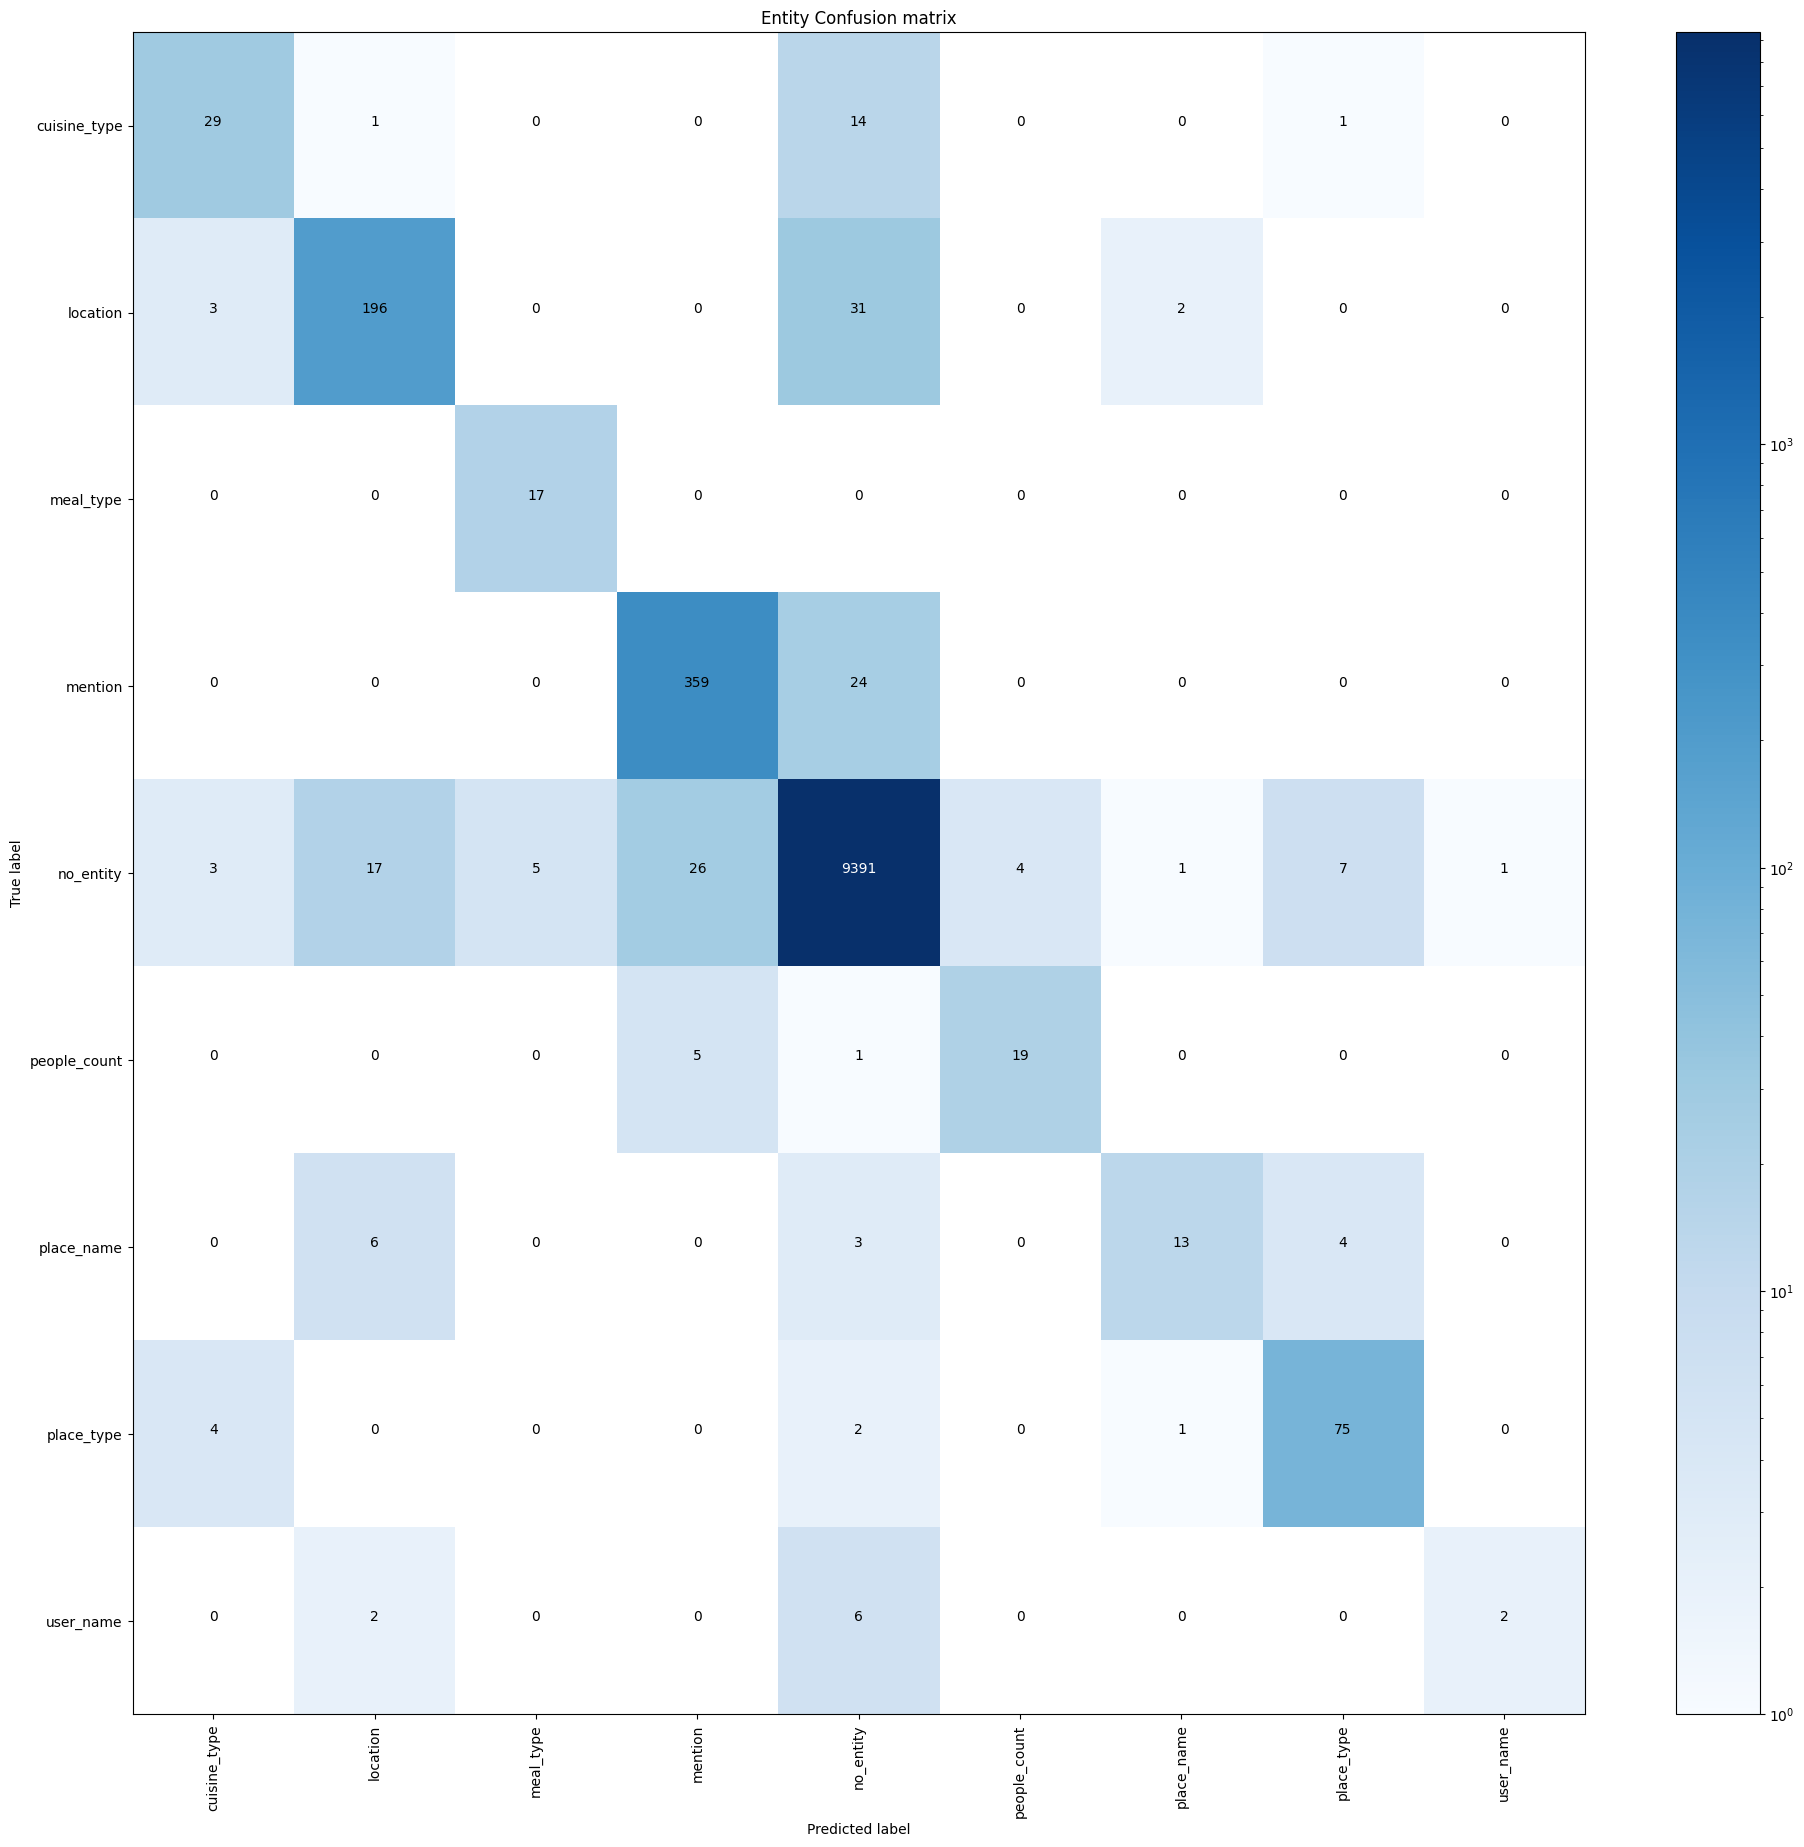
\includegraphics[width=0.8\textwidth]{images/entity_default_cf.png}
    \caption{Confusion matrix for the task of entity classification using the default configuration.}
    \label{fig:entity-default-cf}
\end{figure}

\newpage

\subsection{Dialogue Management Evaluation}

The following figure shows the confusion matrix for the dialogue management model on the test stories. As can be seen, the model correctly predicts all the actions, thus achieving perfect accuracy in the evaluation.

\begin{figure}[h!]
    \centering
    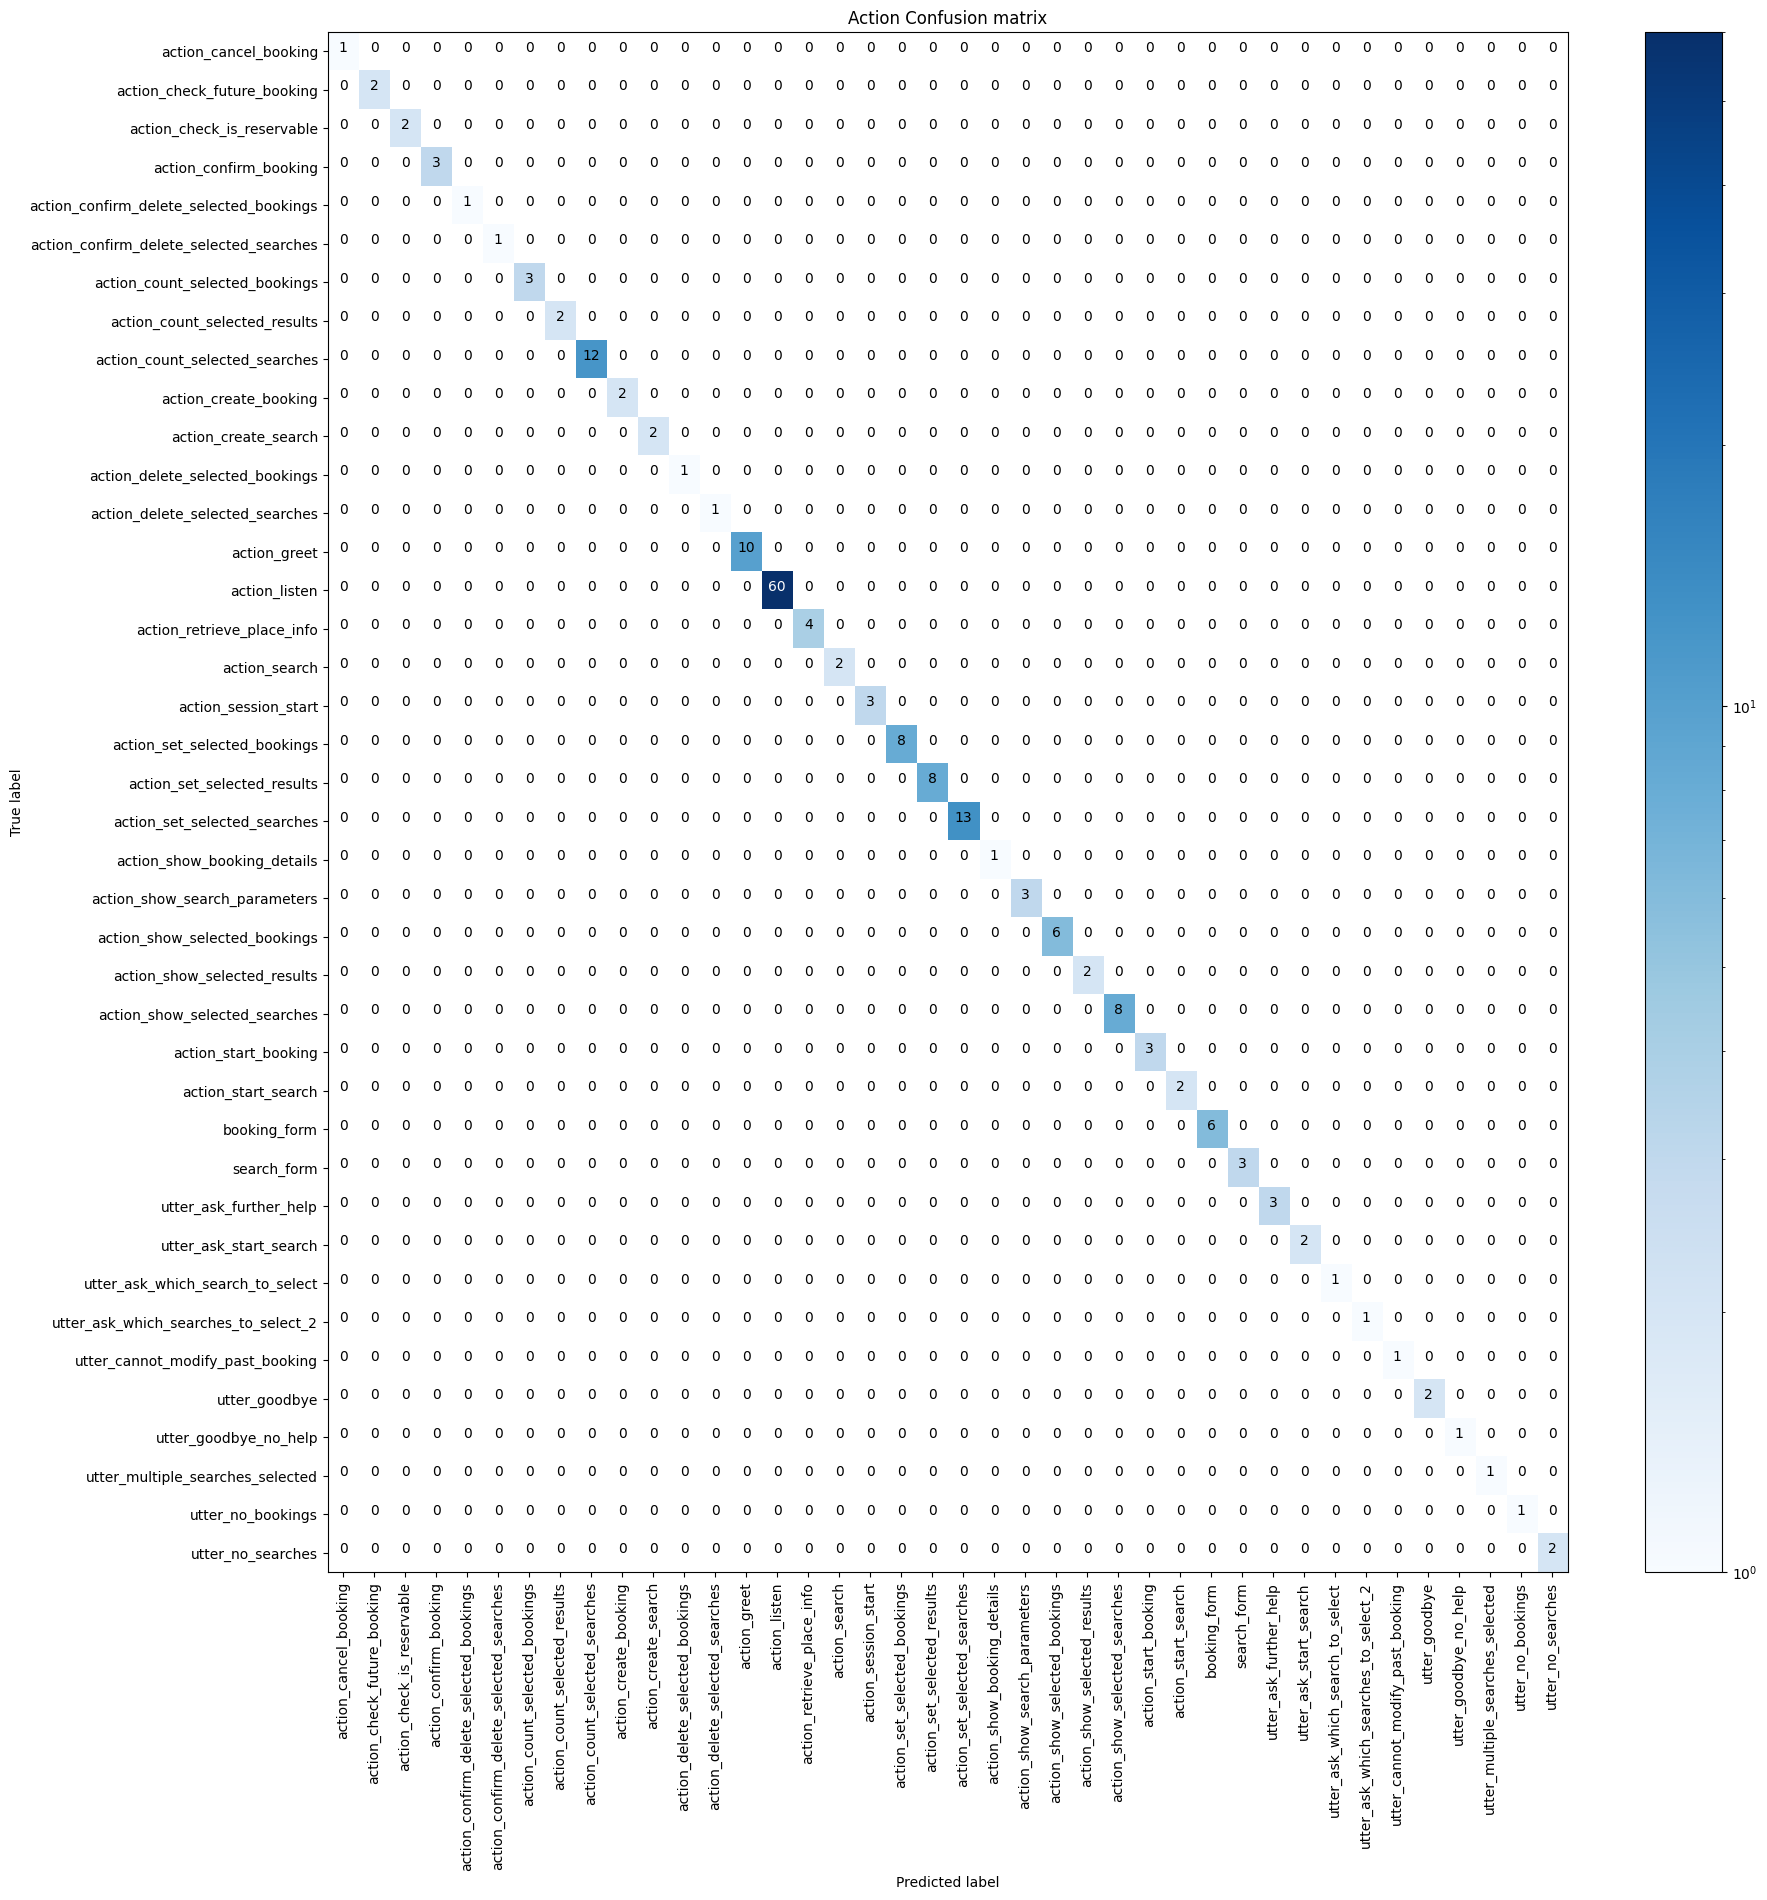
\includegraphics[width=0.8\textwidth]{images/dialogue_cf.png}
    \caption{Confusion matrix for the dialogue management model on the test stories.}
    \label{fig:dialogue-cf}
\end{figure}

\newpage

\subsection{Extrinsic Evaluation}

In Table \ref{tab:extrinsic-evaluation}, the list of questions asked to the participants during the extrinsic evaluation is reported. The participants were asked to rate their satisfaction with the assistant on a scale from 1 to 5, with 1 being very dissatisfied and 5 being very satisfied.

\begin{figure}[h!]
    \centering
    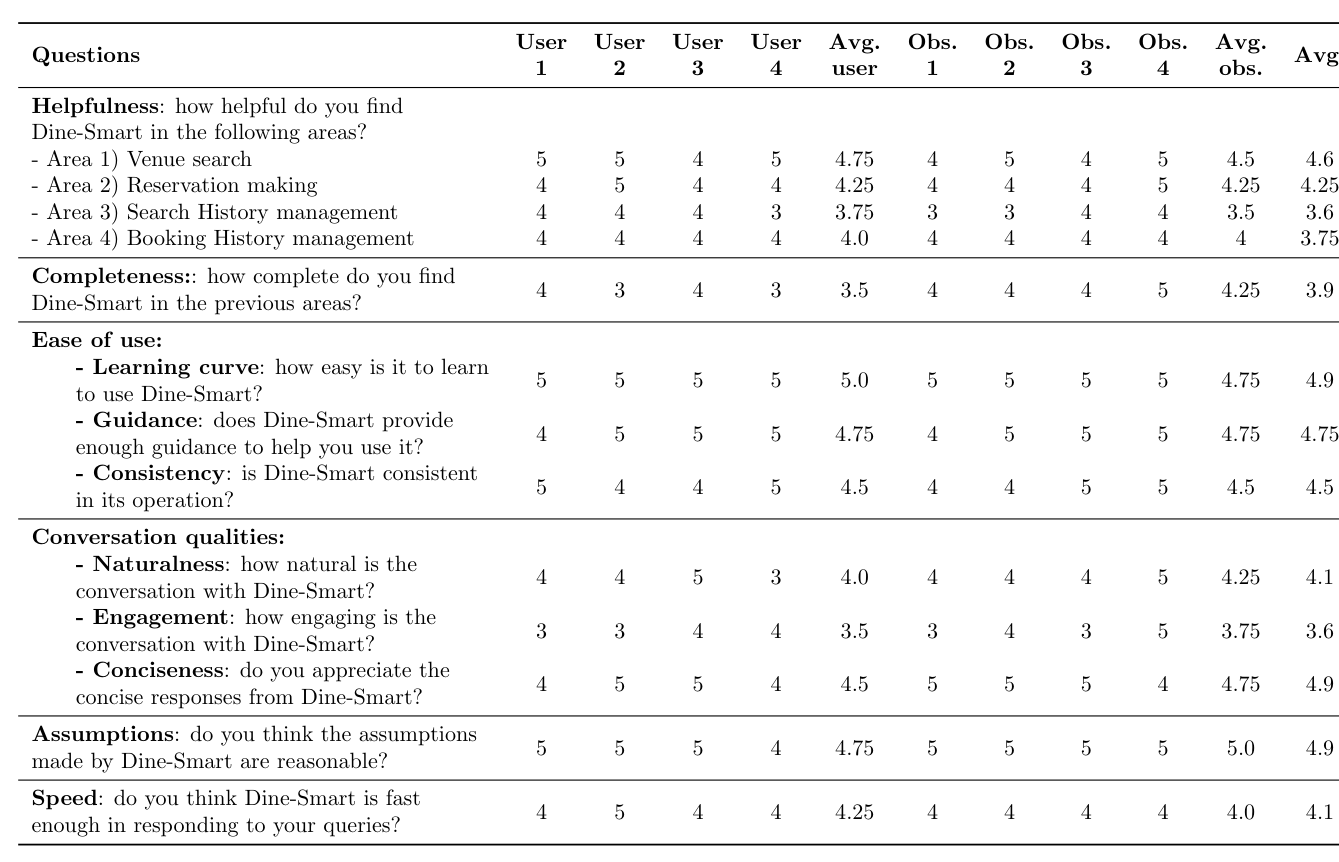
\includegraphics[width=1.0\textwidth]{images/extrinsic.png}
    \caption{Questions and ratings for the extrinsic evaluation.}
    \label{tab:extrinsic-evaluation}
\end{figure}

\end{document}